\documentclass{article}
\usepackage{parskip}
\usepackage{amsmath}
\usepackage[dvipdfmx]{graphicx}
\begin{document}

所与の整数$A, B, C, D, E$は相異なるので,3数の選び方は10通りあり、
選ぶ数を1個だけ変えたものとの大小関係をグラフに表すと下図のようになる。
よって、求める値は$\max \{ E + D + A, E + C + B \}$である。

\vspace{20pt}
\begin{center}
    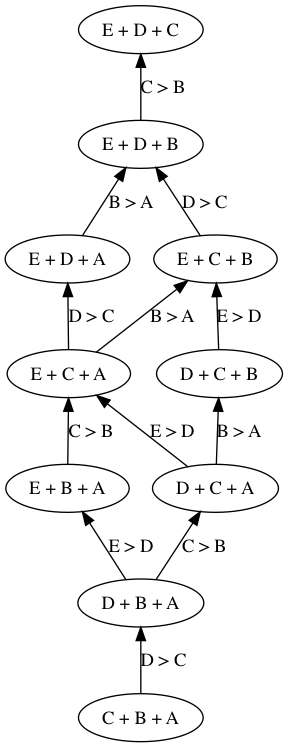
\includegraphics[width=150pt]{graph.png}
\end{center}

\end{document}
